\let\negmedspace\undefined
\let\negthickspace\undefined
\documentclass[journal]{IEEEtran}
\usepackage[a5paper, margin=10mm, onecolumn]{geometry}
\usepackage{lmodern} 
\usepackage{tfrupee} 

\setlength{\headheight}{1cm} % Set the height of the header box
\setlength{\headsep}{0mm}     % Set the distance between the header box and the top of the text

\usepackage{gvv-book}
\usepackage{gvv}
\usepackage{cite}
\usepackage{amsmath,amssymb,amsfonts,amsthm}
\usepackage{algorithmic}
\usepackage{graphicx}
\usepackage{textcomp}
\usepackage{xcolor}
\usepackage{txfonts}
\usepackage{listings}
\usepackage{enumitem}
\usepackage{mathtools}
\usepackage{gensymb}
\usepackage{comment}
\usepackage[breaklinks=true]{hyperref}
\usepackage{tkz-euclide} 
\usepackage{listings}                                      
\def\inputGnumericTable{}                                 
\usepackage[latin1]{inputenc}                                
\usepackage{color}                                            
\usepackage{array}                                            
\usepackage{longtable}
\usepackage{multicol}
\usepackage{calc}                                             
\usepackage{multirow}                                         
\usepackage{hhline}                                           
\usepackage{ifthen}                                           
\usepackage{lscape}
\begin{document}

\bibliographystyle{IEEEtran}
\vspace{3cm}

\title{4.13.36}
\author {EE25BTECH11031 - Sai Sreevallabh}
% \maketitle
% \newpage
% \bigskip
{\let\newpage\relax\maketitle}

\renewcommand{\thefigure}{\theenumi}
\renewcommand{\thetable}{\theenumi}
\setlength{\intextsep}{10pt} % Space between text and floats


\numberwithin{equation}{enumi}
\numberwithin{figure}{enumi}
\renewcommand{\thetable}{\theenumi}

\textbf{Question: }\\

Let $PQR$ be a right angled isosceles triangle, right at $P(2, 1)$. If the equation of the line $QR$ is $2x + y = 3$, then the equation representing the pair of lines $PQ$ and $PR$ is 
    
\begin{multicols}{2}
    \begin{enumerate}
        \item $3x^2 - 3y^2 + 8xy + 20x + 10y + 25 = 0$
        \item $3x^2 - 3y^2 + 8xy - 20x - 10y + 25 = 0$
        \item $3x^2 - 3y^2 + 8xy + 10x + 15y + 20 = 0$
        \item $3x^2 - 3y^2 - 8xy - 10x - 15y - 20 = 0$
    \end{enumerate}
\end{multicols}


\textbf{Solution: }\\

Given point is $\vec{P} = \myvec{2\\1}$ and given line can be written as 
\begin{align}
    \vec{n}^\top\vec{x} = c \label{eq1}
\end{align}

where, $\vec{n} = \myvec{2\\1}$ and $c = 3$.\\

Parametric form of line through $\vec{P}$ is 
\begin{align}
    \vec{r} = \vec{P} + \lambda\vec{m}
\end{align}

Using this, we can represent points $Q$ and $R$ as
\begin{align}
    \vec{Q} = \vec{P} + \lambda_1\vec{m_1}\label{eq3}
\end{align}

\begin{align}
    \vec{R} = \vec{P} + \lambda_2\vec{m_2} \label{eq4}
\end{align}

where, $\vec{m_1} = \myvec{1\\m_1}$ and $\vec{m_2} = \myvec{1\\m_2}$ are direction vectors of lines $\vec{Q-P}$ and $\vec{R-P}$, while $m_1$ and $m_2$ are the respective slopes.\\
%and $\vec{m_2} = \myvec{1\\m_2}$ is the direction vector of line $\vec{PR}$ and $m_2$ is the slope.\\ 

Given that the lines are perpendicular, 
\begin{align}
    \vec{m_1}^\top\vec{m_2} =& 0\\
    \implies m_1m_2 =& -1
\end{align}

Substituting equation \eqref{eq3} in \eqref{eq1}
\begin{align}
    \vec{n}^\top\brak{\vec{P} + \lambda_1\vec{m_1}} = c\\
    \implies \lambda_1 \ = \ \frac{c-\vec{n}^\top\vec{P}}{\vec{n}^\top\vec{m_1}}
\end{align}

Substituting the values, we get
\begin{align}
    \lambda_1 \ = \ \frac{-2}{2+m_1} \label{eq9}
\end{align}

Similarly, substituting equation \eqref{eq4} in \eqref{eq1}
\begin{align}
    \lambda_2 \ = \ \frac{c-\vec{n}^\top\vec{P}}{\vec{n}^\top\vec{m_2}}
\end{align}

Substituting values,
\begin{align}
    \lambda_2 \ =&\ \frac{-2}{2+m_2}
\end{align}

\begin{align}
    \implies \lambda_2 \ =& \ \frac{-2m_1}{2m_1-1} \label{eq12}
\end{align}\\


Let $\vec{M}$ be the midpoint of $\vec{Q-R}$:
\begin{align}
    \vec{M} = \frac{\vec{Q+R}}{2}
\end{align}

Since $\triangle PQR$ is isosceles,
\begin{align}
    \vec{P}-\vec{M} \perp \vec{Q}-\vec{R}\\
    \implies \brak{\vec{P}-\frac{\vec{Q+R}}{2}}^\top \brak{\vec{Q}-\vec{R}} = 0
\end{align}\\

Substituting values from \eqref{eq3}, \eqref{eq4}, we get
\begin{align}
    \brak{\lambda_1\vec{m_1}+\lambda_2\vec{m_2}}^\top\brak{\lambda_1\vec{m_1}-\lambda_2\vec{m_2}} =& 0\\
    \lambda_1^2\vec{m_1}^\top\vec{m_1} =& \lambda_2\vec{m_2}^\top\vec{m_2}\\
    \lambda_1^2\brak{1+m_1^2} =& \lambda_2\brak{1+\frac{1}{m_1^2}}\\
    \abs{\lambda_1}=& \abs{\frac{\lambda_2}{m_1}}
\end{align}\\

Substituting values of $\lambda_1$ and $\lambda_2$ from \eqref{eq9} and \eqref{eq12}

\begin{align}
    \abs{ \frac{2}{2+m_1}} =& \abs{\frac{2}{2m_1-1}}
\end{align}

% Given that the triangle is isosceles,
% \begin{align}
%   \norm{\vec{Q}-\vec{P}}=&\norm{\vec{R-P}}\\
%   \implies \abs{\lambda_1}\norm{\vec{m_1}} =& \abs{\lambda_2}\norm{\vec{m_2}}\\
%   \implies \abs{ \frac{-2}{2+m_1}}\sqrt{1+m_1^2} \ =&\  \abs{\frac{-2m_1}{2m_1-1}}\sqrt{1+\brak{\frac{-1}{m_1}}^2} \\
%   \implies  \abs{ \frac{2}{2+m_1}} =& \abs{\frac{2}{2m_1-1}}
% \end{align}\\

 

Solving the above, we get
\begin{align}
    m_1 = 3 \ \text{or} \ m_1 = \frac{-1}{3}
\end{align}

Correspondingly,
\begin{align}
    m_2 = \frac{-1}{3} \ \text{or} \ m_2 = 3
\end{align}\\

So, the equations of the two required lines are
\begin{align}
    3x-y-5=0 \ \ \text{and}\ \ x+3y-5=0
\end{align}\\

$\therefore$ Multiplying the above two equations, we get the pair of straight lines to be 
\begin{center}
   $3x^2 - 3y^2 + 8xy - 20x - 10y + 25 = 0$
\end{center} 

\begin{figure}[H]
    \centering
    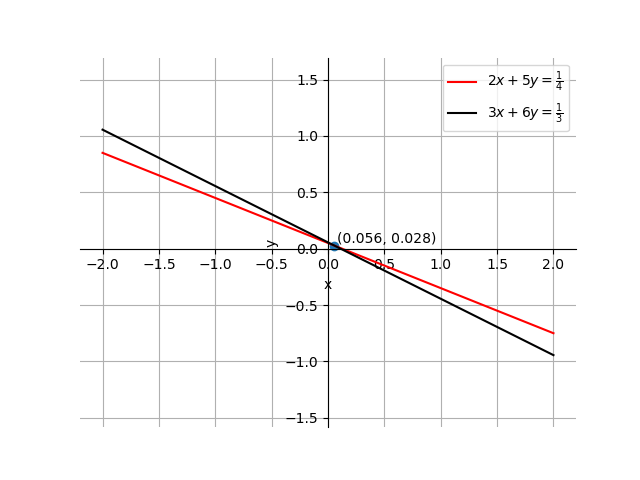
\includegraphics[width=1\linewidth]{Figs/plot(py).png}
\end{figure}

\end{document}
